

\begin{figure}
\begin{center}
\resizebox{3in}{!}{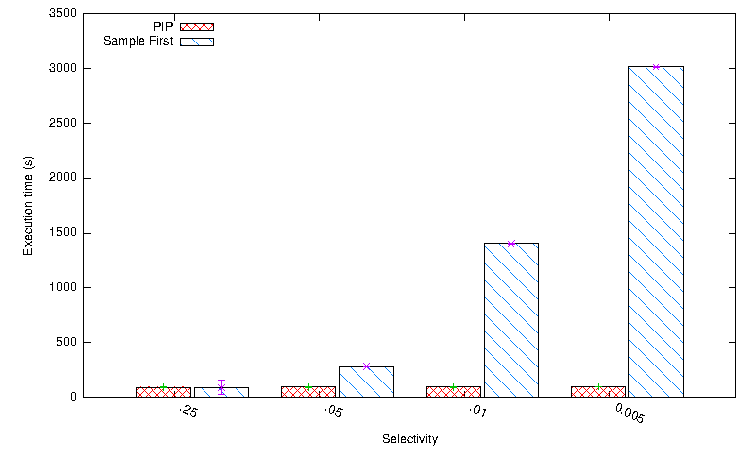
\includegraphics{graphics/scaling_selectivity.pdf}}
\caption{Time to complete a 1000 sample query, accounting for selectivity-induced loss of accuracy.}
\label{fig:scaling_selectivity}
\end{center}
\end{figure}


\begin{figure}
\begin{center}
\resizebox{3in}{!}{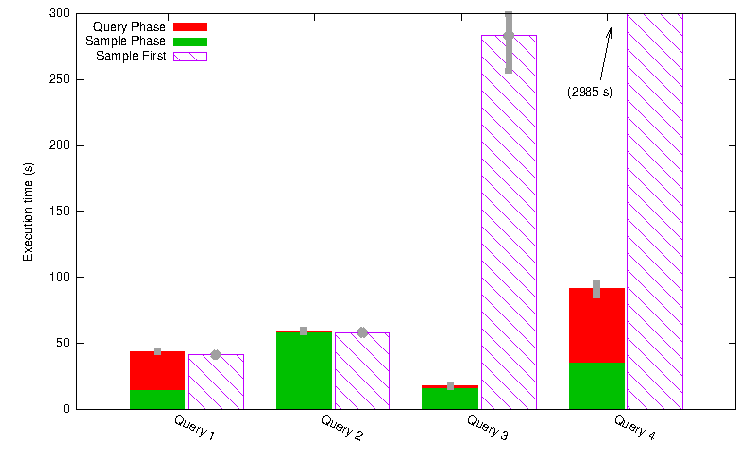
\includegraphics{graphics/query_timings.pdf}}
\caption{Query evaluation times in PIP and Sample-First for a range of queries.  Sample-First's sample-count has been adjusted to match PIP's accuracy.}
\label{fig:querytimings}
\end{center}
\end{figure}

\begin{figure*}
\begin{center}
\subtable[]{\resizebox{3in}{!}{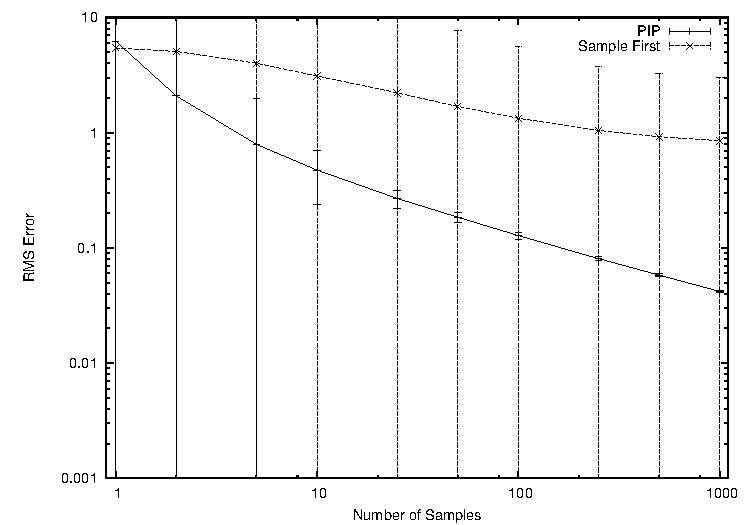
\includegraphics{graphics/variance.pdf}} \label{subfig:variance1}}
\subtable[]{\resizebox{3in}{!}{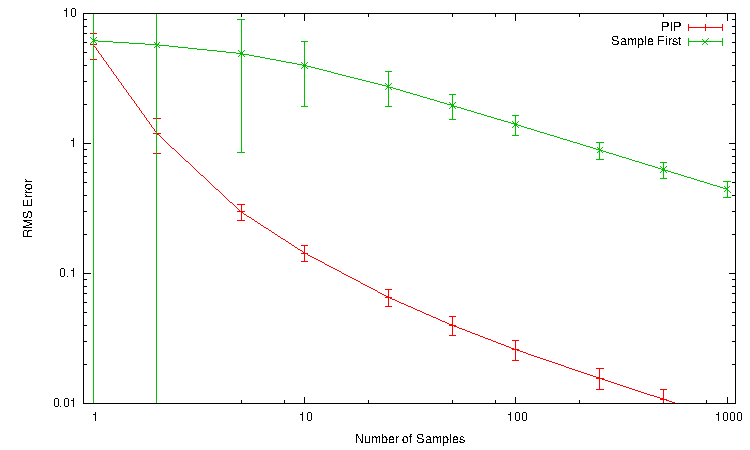
\includegraphics{graphics/variance2.pdf}}\label{subfig:variance2}}
\vspace*{-0.1in}
\caption{RMS error across the results of 30 trials of (a) a simple group-by query $Q_4$ with a selectivity of $0.005$, and (b) a complex selection query $Q_5$ with an average selectivity of $0.05$.}
\label{fig:variance}
\end{center}
\vspace*{-0.20in}
\end{figure*}

As a comparison point for PIP's ability to manage continuous random variables, we have constructed a sample-first probabilistic extension to Postgres that emulates MCDB's tuple-bundle concept using ordinary Postgres rows.  A sampled variable is represented using an array of floats, while the tuple bundle's presence in each sampled world is represented using a densely packed array of booleans.  In lieu of an optimizer, test queries were constructed by hand so as to minimize the lifespan of either array type.

Using Postgres as a basis for both implementations places them on an equal footing with respect to DBMS optimizations unrelated to probabilistic data.  This makes it possible to focus our comparison solely on the new, probabilistic functionality of both systems.  However, to make the distinction from MCDB (which is a separate development not based on Postgres) explicit, we refer to our implementation of the MCDB approach as Sample-First.

We evaluated both the PIP C-Tables and the Sample-First infrastructure against a variety of related queries.  Tests were run over a single connection to a modified instance of PostgreSQL 8.3.4 with default settings running on a 2x4 core 2.0 GHz Intel Xeon with a 4MB cache.  Unless otherwise specified queries were evaluated over a 1 GB database generated by the TPC-H benchmark, all sampling processes generate 1000 samples apiece, and results shown are the average of 10 sequential trials with error bars indicating one standard deviation.

First, we demonstrate PIP's performance on a simple set of queries ideally suited to the strengths of Sample-First.  These two queries (identical to Q1 and Q2 from \cite{MCDB}) involve pa\-ra\-me\-tri\-zing a table of random values, applying a simple set of math operations to the values, and finally estimating the sum of a large aggregate over the table.  

The first query computes the rate at which customer purchases have increased over the past two years.  The percent increase parametrizes a Poisson distribution that is used to predict how much more each customer will purchase in the coming year.  Given this predicted increase in purchasing, the query estimates the company's increased revenue for the coming year.

In the second query, past orders are used to compute the mean and standard deviation of manufacturing and shipping times.  These values parametrize a pair of Normal distributions that combine to predict delivery dates for each part ordered today from a Japanese supplier.  Finally, the query computes the maximum of these dates, providing the customer with an estimate of how long it will take to have all of their parts delivered.

The results of these tests are shown as query $Q_1$ and $Q_2$, respectively, in Figure \ref{fig:querytimings}.  Note that performance times for PIP are divided into two components: query and sample, to distinguish between time spent evaluating the deterministic components of a query and building the result c-table, and time spent computing expectations and confidences of the results.  The results are positive; the overhead of the added infrastructure is minimal, even on queries where Sample-First is sufficient.  Furthermore, especially in Q2, the sampling process comprises a relatively small portion of the query; additional samples can be generated without incurring the nearly 1 minute query time.

The third query $Q_3$ in Figure \ref{fig:querytimings} combines a simplified form of queryies $Q_1$ and $Q_2$.  Rather than aggregating, the query compares the delivery times of $Q_2$ to a set of ``satisfaction thresholds."  This comparison results in a (probabilistic) table of dissatisfied customers that is used in conjunction with $Q_1$'s profit expectations to estimate profit lost to dissatisfied customers.  A query of this form might be run on a regular basis, perhaps even daily.  As per this usage pattern, we pre-materialize the component of this query unlikely to change on a daily basis: the expected shipping time parameters.

%  $Q_3$ is described in more detail in the Appendix Section \ref{sec:timingq3}

Though PIP and Sample-First both take the same amount of time to generate 1000 samples under this query, the query's selectivity causes Sample-First to disregard a significant fraction of the samples generated; for the same amount of work, Sample-First generates a less accurate answer.  To illustrate this point, see Figure \ref{subfig:variance1}.  This figure shows the RMS error, normalized by the correct value in the results of a query for predicted sales of 5000 parts in the database, given a Poisson distribution for the increase in sales and a popularity multiplier chosen from an exponential distribution.  As an additional restriction, the query considers only the extreme scenario where the given product has become extremely popular (resulting in a selectivity of $e^{-5.29} \approx 0.005$).  

RMS error was computed over 30 trials using the algebraically computed correct value as a mean, and then averaged over all 5000 parts.  Note that PIP's error is over two orders of magnitude lower than the sample-first approach for a comparable number of samples.  This corresponds to the selectivity of the query; as the query becomes more selective, the sample-first error increases.  Furthermore, because CDF sampling is used to restrict the sampling bounds, the time taken by both approaches to compute the same number of samples is equivalent.

A similar example is shown in Figure \ref{subfig:variance2}.  Here, a model is constructed for how much product suppliers are likely to be able to produce in the coming year based on an Exponential distribution, and for how much product the company expects to sell in the coming year as in Q1.  From this model, the expected underproduction is computed, with a lower bound of 0; the selection criterion considers only those worlds where demand exceeds supply.  For the purposes of this test, the model was chosen to generate an average selectivity of 0.05.  Though the comparison of 2 random variables necessitates the use of rejection sampling and increases the time PIP spends generating samples, the decision to drop a sample is made immediately after generating it; PIP can continue generating samples until it has a sufficient number, while the Sample-First approach must rerun the entire query.

Note the relatively large variance in the RMS error of the Sample-First results these figures, particularly the first one.  Here, both the selectivity and the price for each part vary with the part.   Thus, some parts become more important while others become harder to sample from.  In order to get a consistent answer for the entire query Sample-First must provision enough samples for the worst case, while PIP can dynamically scale the number of samples required for each term.

Returning to Figure \ref{fig:querytimings}, Queries $Q_3$ and $Q_4$ have been run with PIP at a fixed 1000 samples.  As Sample-First drops all but a number of samples corresponding to the selectivity of the query, we run Sample-First with a correspondingly larger number of samples.  For Query 3, the average selectivity of 0.1 resulted in Sample-First discarding 10\% of its samples.  To maintain comparable accuracies, Sample-First was run at 10,000 samples.  

We expand on this datapoint in Figure \ref{fig:scaling_selectivity} where we evaluate $Q_4$, altered to have varying selectivities.  The sample-first tests are run with $\frac{1}{selectivity}$ times as many samples as PIP to compensate for the lower error, in accordance with Figure \ref{subfig:variance1}.  Note that selectivity is a factor that a user must be aware of when constructing a query with sample-first while PIP is able to account for selectivity automatically, even if rejection sampling is required.

It should also be noted that both of these queries include two distinct, independent variables involved in the expectation computation.  A studious user may note this fact and hand optimize the query to compute these values independently.  However, without this optimization, a sample-first approach will generate one pair of values for each customer for each world.  As shown in the RMS error example, an arbitrarily large number of customer revenue values will be discarded and the query result will suffer.  In this test, customer satisfaction thresholds were set such that an average of 10\% of customers were dissatisfied.  Consequently sample-first discarded an average of 10\% of its values.  To maintain comparable accuracies, the sample-first query was evaluated with 10,000 samples while the PIP query remained at 1000 samples. 

As a final test, we evaluated both PIP and our Sample-First implementation on the NSIDC's Iceberg Sighting Database\cite{iceberg} for the past 4 years.  100 virtual ships were placed at random locations in the North Atlantic, and each ship's location was evaluated for its proximity to potential threats; Each iceberg in the database was assigned a normally distributed position relative to its last sighting, and an exponentially decaying danger level based on time since last sighting.  Recently sighted icebergs constituted a high threat, while historic sightings represented potential new iceberg locations.  The query identified icebergs with greater than a 0.1\% chance of being located near the ship and estimated the total thret posed by all potentially nearby icebergs.  The results of this experiment are shown in Figure \ref{fig:iceberg}\footnote{Due to time constraints, this graph only contains the results of 6 runs.  The camera-ready version will express the full 10 runs}.  PIP was able to employ CDF sampling and obtain an exact result within 10 seconds.  By comparison, the Sample-First implementation generating 10,000 samples took over 10 minutes and produced results deviating by as much as 25\% from the correct result on average.

\begin{figure}
\begin{center}
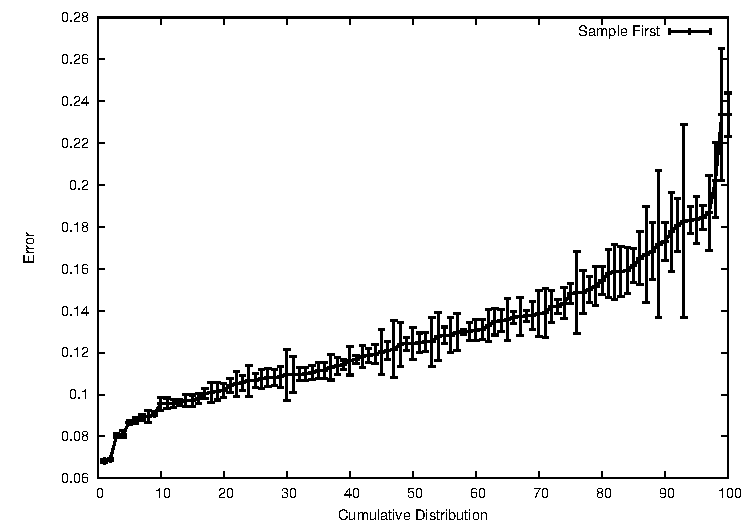
\includegraphics[width=3in]{graphics/iceberg_danger.pdf}
\caption{Sample-First error as a fraction of the correct result in a danger-estimation query on the NSIDC's Iceberg Sighting Database.  PIP was able to obtain an exact result.}
\end{center}
\label{fig:iceberg}
\vspace*{-0.3in}
\end{figure}

%\begin{figure}
%\begin{center}
%\resizebox{3in}{!}{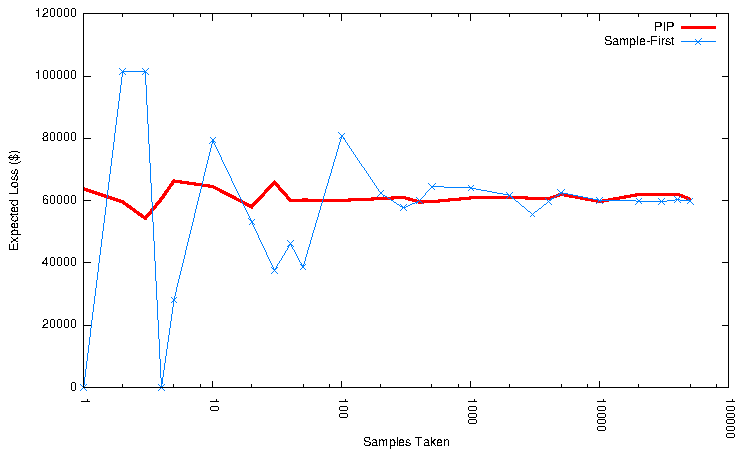
\includegraphics{graphics/iterative_refinement.pdf}}
%\caption{Variance as a function of samples in PIP and Sample-First.  Each data point is an estimate generated by a single run at the indicated number of samples}
%\label{fig:iterativerefinement}
%\end{center}
%\end{figure}
%
%
%Figure \ref{fig:iterativerefinement} demonstrates one extreme case of this in a comparison between Karp-Luby estimates and Sample-First estimates.  The results shown are for repeated executions of a query similar to query 4, save with a filter that removes all but approximately 10 clients.  In queries that do not involve a large linear aggregate, the sample-first approach disqualifies a sufficient number of possible worlds that subsequent expectation computations falter.  Conversely the Karp-Luby estimator has sufficient information that it can employ a precomputed CDF lookup table to compute each row's bag probabilities.  Because of this and the fact that it generates more ``useful'' samples, its results have a much lower variance with far fewer samples required.
